%%%%%%%%%%%%%%%%%%%%%%%%%%%%%%%%%%%%%%
% LaTeX poster template
% Created by Nathaniel Johnston
% August 2009
% http://www.nathanieljohnston.com/2009/08/latex-poster-template/
%%%%%%%%%%%%%%%%%%%%%%%%%%%%%%%%%%%%%%

\documentclass[final]{beamer}
\usepackage[scale=1.24]{beamerposter}
\usepackage{graphicx}			% allows us to import images
\usepackage{oz}

%-----------------------------------------------------------
% Define the column width and poster size
% To set effective sepwid, onecolwid and twocolwid values, first choose how many columns you want and how much separation you want between columns
% The separation I chose is 0.024 and I want 4 columns
% Then set onecolwid to be (1-(4+1)*0.024)/4 = 0.22
% Set twocolwid to be 2*onecolwid + sepwid = 0.464
%-----------------------------------------------------------

\newlength{\sepwid}
\newlength{\onecolwid}
\newlength{\twocolwid}
\newlength{\threecolwid}
\setlength{\paperwidth}{48in}
\setlength{\paperheight}{36in}
\setlength{\sepwid}{0.024\paperwidth}
\setlength{\onecolwid}{0.22\paperwidth}
\setlength{\twocolwid}{0.464\paperwidth}
\setlength{\threecolwid}{0.708\paperwidth}
\setlength{\topmargin}{-0.5in}
\usetheme{confposter}
\usepackage{exscale}

%-----------------------------------------------------------
% The next part fixes a problem with figure numbering. Thanks Nishan!
% When including a figure in your poster, be sure that the commands are typed in the following order:
% \begin{figure}
% \includegraphics[...]{...}
% \caption{...}
% \end{figure}
% That is, put the \caption after the \includegraphics
%-----------------------------------------------------------

\usecaptiontemplate{
\small
\structure{\insertcaptionname~\insertcaptionnumber:}
\insertcaption}

%-----------------------------------------------------------
% Define colours (see beamerthemeconfposter.sty to change these colour definitions)
%-----------------------------------------------------------

\setbeamercolor{block title}{fg=black,bg=white}
\setbeamercolor{block body}{fg=black,bg=white}
\setbeamercolor{block alerted title}{fg=white,bg=norange!60}
\setbeamercolor{block alerted body}{fg=black,bg=dblue!10}

%-----------------------------------------------------------
% Name and authors of poster/paper/research
%-----------------------------------------------------------

\title{Coupled Electric Oscillators}
\author{Trevor Smith, Alex Storrer}
\institute{Physics Department of Northeastern University}

%-----------------------------------------------------------
% Start the poster itself
%-----------------------------------------------------------

\begin{document}
\begin{frame}[t]
  \begin{columns}[t]					% the [t] option aligns the column's content at the top

    \begin{column}{\sepwid}\end{column}
    \begin{column}{\onecolwid}					  % create a three-column-wide column and then we will split it up later
	    \begin{block}{Abstract}

		    First we analyze a single LRC circuit.
		    By curve fitting voltage responses for the circuit,
		    the A and B-inductor
		    decay natural frequencies is calculated as 14587.05$\pm$
		    0.03  rad/sec and 14578.44$\pm$ 0.03 rad/s, and decay constants of
		    649.9$\pm$ 0.1 $s^{-1}$ and 651.3$\pm$ 0.1 $s^{−1}$.  From these values the
		    inductances is calculated to be 0.100±0.003 H for both of the inductors.
		    When the A and B circuits were coupled via a coupling capacitor, each
		    circuit produced a signal with a beat frequency of 170 $\pm$ 1 Hz.
		    By using equations modeling a coupled LRC circuit, the coupling
		    capacitance is calculated to be 4.1 $\pm$ 0.1 nF, which is one standard
		    deviation away from its measured value of 3.9 $\pm$ 0.1 nF.

	    \end{block}

	    \vskip2ex

      \begin{block}{Introduction}
	Three essential components used in circuits are resistors, 
	capacitors, and inductors. These components operate in distinct ways, which can be
	seen by the way we use inductance, resistance, and capacitance to calculate voltage.

	\vskip1ex

	\begin{alertblock}{Equations for Voltage}
		\begin{semiverbatim}
		$$ V = L \cdot \frac{d^2q}{dt^2} \fcmp\ \  V = R \cdot \frac{dq}{dt} \fcmp\ \  V = \frac{1}{C} \cdot q $$
		\end{semiverbatim}
	\end{alertblock}

	\vskip0ex
	Where V is voltage, L is inductance, R is resistance, C is capacitance, and q is 
	charge. In other words, capacitors do work proportional to amount of charge buildup, 
	resistors do work proportional to the flow of charge or current, and inductors do 
	work proporional to the inflection of charge, or the change in current. \\
	\vskip1ex

	\vskip1ex
	An LRC circuit combines these three components in series, and produces damped
	oscillation in response to changing voltage, via the above equations and
	Kirchoff's loop rule.
	We can understand why by relating these oscillations analagous to a spring-mass system.
	\vskip1ex

	\end{block}


    \end{column}

    \begin{column}{\sepwid}\end{column}			% empty spacer column
    \begin{column}{\onecolwid}
    \begin{block}{Introduction, cont.}

	\setbeamercolor{block alerted title}{fg=black,bg=nblue!60}	% frame color
	\begin{alertblock}{ }
	\begin{figure}[h]
	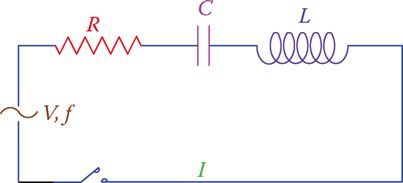
\includegraphics[width=0.5\textwidth]{../Images/l6_LRC.jpg}
	\caption{\label{figA} An LRC Circuit}
	\end{figure}
	\end{alertblock}

	\setbeamercolor{block alerted title}{fg=white,bg=norange!60}	% frame color
	\begin{alertblock}{Differential Equations}
		\begin{semiverbatim}
		$$ L \cdot \frac{d^2q}{dt^2} + R \cdot \frac{dq}{dt} + \frac{1}{C} \cdot q = 0 $$
		$$ m \cdot \frac{d^2x}{dt^2} + \beta \cdot \frac{dx}{dt} + kx = 0 $$
		\end{semiverbatim}
	\end{alertblock}

	These circuits grow exponentially in complexity when two are copuled 
	together. In the second phase of this lab we investigate the behavior
	of two coupled LRC circuits, operating with a 90 degree phase difference.

      \end{block}

      \begin{block}{Apparatus}
% List equipment components (manufacturer, model
% numbers and brief specifications). 

The apparatus consisted of the following.
\begin{itemize}
	\item Coupled electronic oscillator circuit box
	\item Fixed capacitor, variable capacitor
	\item Two large inductor coils, labelled 'A' and 'B'
	\item Oscilloscope, Tektronix TDS210 
	\item Digital Multimeter, Extech EX430A
\end{itemize}

\end{block}

\begin{block}{Measure Inductance}

	In this phase of the lab we measure the basic parameters of our system, described
	in fig. \ref{setup}, including $L_A$, $L_B$, $R_L_A$, $R_L_B$, full decay natural 
	frequency $\omega_0$, damping constant $\gamma$, time constant $\tau$, 
	quality factor $Q$ and the standard capacitor. These values, save for the capacitance,
	are calculated by analyzing the voltage oscillations of the circuit. Values for $R_L_A$
	and $R_L_B$ are also measured with an ohmmeter, and the capacitance is measured
	with a digital multimeter (DMM). \\

\end{block}

\end{column}
  

    \begin{column}{\sepwid}\end{column}			% empty spacer column
    \begin{column}{\onecolwid}					  % create a three-column-wide column and then we will split it up later

\begin{block}{Measure Inductance, cont.}

	\setbeamercolor{block alerted title}{fg=black,bg=nblue!60}	% frame color
	\begin{alertblock}{ }
	\begin{figure}[h]
	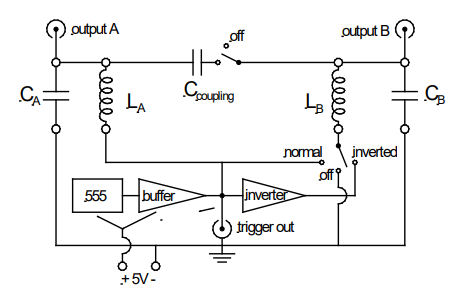
\includegraphics[width=0.85\textwidth]{../Images/l6_setup.png}
	\caption{\label{setup} Test setup for the coupled electric oscillators.}
	\end{figure}
	\end{alertblock}

	The fit parameters will correspond to this solution of an LRC circuit.

	\begin{equation} 
	q(t) = q_{0}e^{-\gamma t/2}cos(\omega_0t)
	\label{LRC Oscillation}
	\end{equation}

	\vskip1ex

	\setbeamercolor{block alerted title}{fg=black,bg=nblue!60}	% frame color
	\begin{alertblock}{ }
	\begin{figure}[h]
	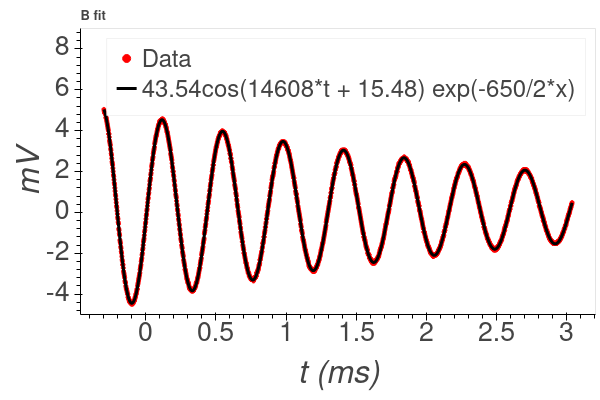
\includegraphics[width=0.85\textwidth]{../Images/l6_channel_B_full_fit.png}
	\caption{\label{single_period} LRC Circuit response and fit, using B-inductor.
	The sign of the frequency is not relevant in this case. }
	\end{figure}
	\end{alertblock}
		
	The fit matched the data extremely well.
	The measuring precision of the DMM is responsible for virtually
	all uncertainty in calculated values in this lab.

\end{block}

\vskip2ex

\begin{block}{Coupled Electric Oscillators}

In the following section, a system with two coupled LRC circuits is
analyzed. In this configuration, the square wave only excites
the A-circuit, meaning that at the end of a pulse the A-capacitor
is fully charged and the B-capacitor is empty.
The decay is removed digitally by fitting the sum of both responses,
and dividing each by the exponential, with the result shown in
fig. \ref{waves}

\end{block}

\end{column}

\begin{column}{\sepwid}\end{column}			% empty spacer column
\begin{column}{\onecolwid}


\begin{block}{Coupled Oscillators, cont.}

\setbeamercolor{block alerted title}{fg=black,bg=nblue!60}	% frame color
\begin{alertblock}{ }

	\begin{figure}[h]
	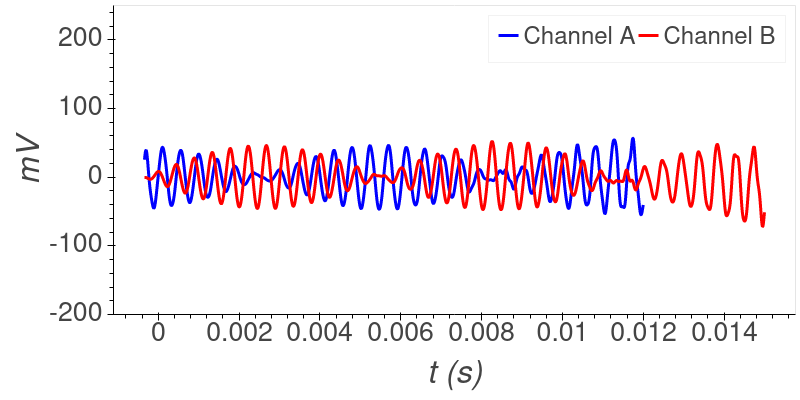
\includegraphics[width=\textwidth]{../Images/l6_channels_sans_decay.png}
	\caption{\label{waves} Two coupled LRC circuits, operating at a 90 degree
	phase difference, with the effect of damping removed.}
	\end{figure}

\end{alertblock}

	The beat frequency of both waves are found using
	two methods of analysis, and the resulting average
	value for each wave is considered. This value was
	the same for both waves, at $170\ \pm\ 1$ Hz.\\

	\vskip1ex
	This value, the difference between $\omega_+$ and 
	$\omega_-$, can be used to calculate the coupling
	capacitance via the following equations, derived
	from differential analysis of the circuit.

\setbeamercolor{block alerted title}{fg=white,bg=norange!60}	% frame color
\begin{alertblock}{ }
	\begin{equation} 
	\omega_+ = \frac{1}{2\pi\sqrt{LC}}
	\label{omegaplus}
	\end{equation}

	\begin{equation} 
	\omega_- = \frac{1}{2\pi\sqrt{L(C+C_{coup})}}
	\label{omegaminus}
	\end{equation}

	\begin{equation} 
	f_{beat} = \frac{1}{2\pi\sqrt{LC}}-\frac{1}{2\pi\sqrt{L(C+2C_{coup})}}
	\label{omegaminus}
	\end{equation}

	\begin{equation} 
	C_{coup} = \frac{1}{2}\left[\frac{1}{L(\frac{1}{\sqrt{LC}}-2\pi f_{beat})^2}-C\right]
	\label{ccoup}
	\end{equation}
\end{alertblock}

\end{block}

\begin{block}{Conclusion}

	The final measured and calculated values for $C_{coup}$ 
	are 3.9 $\pm$ 0.1 nF and 4.1 $\pm$ 0.1 nF respectively,
	which shows agreement within 1 sigma. This shows
	excellent agreement with measured values, and verifies
	the mathematical analysis and digital signal processing
	used to produce the result.

\end{block}

\end{column}

  \begin{column}{\sepwid}\end{column}			% empty spacer column

 \end{columns}

\end{frame}

\end{document}
